\documentclass[11pt,a4paper]{article}
\usepackage[a4paper,margin=2cm]{geometry}
\usepackage[T1]{fontenc}
\usepackage{lmodern}
\usepackage{microtype}
\usepackage{booktabs,tabularx,array}
\usepackage{enumitem}
\usepackage{xcolor}
\usepackage{tikz}
\usetikzlibrary{arrows.meta,positioning,fit,backgrounds,calc}
\usepackage[most]{tcolorbox}
\usepackage[hidelinks]{hyperref}
\usepackage{titlesec}
\usepackage{float}
\usepackage{caption}
\captionsetup{font=small,labelfont=bf,skip=3pt}

\definecolor{accent}{HTML}{1F4E79}
\definecolor{soft}{HTML}{EAF1F8}
\definecolor{toolc}{HTML}{FFF4E0}
\definecolor{safec}{HTML}{FDECEC}
\definecolor{okc}{HTML}{E8F5E9}
\definecolor{specc}{HTML}{F3E8FD}
\definecolor{greyc}{HTML}{F4F4F4}

\titleformat{\section}{\large\bfseries\color{accent}}{\thesection}{0.6em}{}
\titlespacing*{\section}{0pt}{7pt}{2pt}
\titleformat{\subsection}{\normalsize\bfseries}{\thesubsection}{0.5em}{}
\titlespacing*{\subsection}{0pt}{4pt}{1pt}
\setlist{nosep,leftmargin=1.2em}
\setlength{\parindent}{0pt}
\setlength{\parskip}{3pt}
\renewcommand{\arraystretch}{1.12}
\newcolumntype{L}{>{\raggedright\arraybackslash}X}

\newtcolorbox{keybox}[1][]{colback=soft,colframe=accent,boxrule=0.6pt,arc=2pt,
  left=5pt,right=5pt,top=3pt,bottom=3pt,fonttitle=\bfseries,#1}

\tikzset{
  box/.style={draw=accent,fill=soft,rounded corners=2pt,align=center,font=\small,inner sep=3pt,minimum height=8mm},
  tool/.style={draw=orange!70!black,fill=toolc,rounded corners=2pt,align=center,font=\footnotesize,inner sep=2.5pt,minimum height=7mm},
  ok/.style={draw=green!45!black,fill=okc,rounded corners=2pt,align=center,font=\footnotesize,inner sep=2.5pt,minimum height=7mm},
  bad/.style={draw=red!60!black,fill=safec,rounded corners=2pt,align=center,font=\footnotesize,inner sep=2.5pt,minimum height=7mm},
  spec/.style={draw=violet!70!black,fill=specc,rounded corners=2pt,align=center,font=\small,inner sep=3pt,minimum height=8mm},
  kb/.style={draw=black!55,fill=greyc,rounded corners=2pt,align=center,font=\footnotesize,inner sep=2.5pt,minimum height=7mm},
  arr/.style={-{Stealth[length=2.2mm]},thick,accent},
  darr/.style={-{Stealth[length=2mm]},dashed,thick,violet!70!black},
  garr/.style={-{Stealth[length=2mm]},black!55},
}

\begin{document}

%================ TITLE =================
\begin{center}
{\LARGE\bfseries\color{accent} CounselCopilot}\\[3pt]
{\Large\bfseries\color{accent} Catching and Repairing Policy and Legal Conflicts in NDA Drafts\\[1pt]
with Applicability-Aware Retrieval and a Red-Team Repair Loop}\\[6pt]
{\large LMA Group Project 2026 \,--\, Project Proposal}\\[3pt]
\textbf{Team members (roll numbers):}\\[1pt]
2025201049 \qquad 2025201044 \qquad 2025201068 \qquad 2025201038
\end{center}

\begin{keybox}[title=Summary in three lines]
\textbf{Problem:} legal consultants who draft NDAs change often and cannot learn hundreds of pages of company policy, so their drafts quietly \emph{miss} required terms or break rules.\\
\textbf{Idea:} a drafting copilot that finds every company rule and Indian-law provision that \emph{applies to this deal} and checks the draft against each one, citing both sides. It then \emph{hardens} the draft: an opposing-counsel agent hunts for loopholes, a repairer writes minimal redlines, and a regression checker re-runs every rule so that no fix breaks another.\\
\textbf{Test:} on real NDAs with expert-labelled and planted defects, does applicability-aware retrieval catch more omissions with fewer false alarms than standard RAG, long context and checking every rule? And does the red-team loop leave fewer problems and introduce fewer new ones than one-shot repair or self-refine?
\end{keybox}

%================ 1 =================
\section{Domain, target user and problem}
\textbf{Domain:} Legal. \textbf{Scope:} one contract type (NDAs), one jurisdiction (India), three companies' policy packs.\\
\textbf{Target user:} a legal consultant (contract staff, outsourced counsel or junior associate) drafting NDAs for a company, with a senior lawyer who signs off.

\textbf{Problem statement.}
Companies spread their NDA requirements across many documents: data-protection, IP and vendor policies, an approval matrix and past negotiated positions.
The consultants who draft NDAs rotate often, and a new consultant cannot absorb all of this in a few days.
Their typical mistake is not bad wording but a \emph{missing} or non-compliant term, such as no data-return clause, a confidentiality period shorter than policy allows, or a foreign governing law that needs General Counsel approval.
Some drafts also contain terms that are risky under Indian law, such as a broad non-compete, which is void as a restraint of trade under s.27 of the Indian Contract Act, 1872.
These misses surface later as disputes.
A reviewer that reads the draft once cannot find a missing clause, because there is nothing in the text to point at.
We want a copilot that checks every applicable rule, then attacks and repairs the draft the way an experienced opposing lawyer and a senior colleague would, acting as knowledge transfer at the moment the consultant needs it.

\textbf{Why it matters.} NDAs are the most frequently signed contracts, consultant turnover is high, and one missed rule can expose a company's data or IP. A senior lawyer can verify a cited flag in seconds but cannot re-read every policy for every draft.

%================ 2 =================
\section{What is missing in existing approaches}
\begin{itemize}
\item \textbf{Contract-error benchmarks} (CLAUSE, EACL Findings 2026; ContractScrub, 2026) test single prompted models on errors inside one contract; the best macro recall on ContractScrub is only 0.75. \textbf{ContractEval} (NLLP 2025) finds that open models wrongly answer ``no such clause'' in about 25--30\% of cases. None of them checks a draft against a \emph{company's own policies}.
\item \textbf{PolicyGuard} (arXiv 2606.32004, 2026), the closest work, compiles one company's NDA playbook into logic rules and checks every rule. It is evaluated on 5 confidential contracts that cannot be released and ignores deal-specific applicability. Most importantly, it \emph{only flags}: it writes no redlines, and its authors list cross-rule consistency as an open limitation.
\item \textbf{Industry tools} (Harvey, LegalOn, Spellbook) offer ``playbook review'' with private evaluations only. \textbf{There is no open benchmark for policy compliance of NDAs that tests omissions.}
\item \textbf{Adversarial and self-correcting agents.} LegalSim (NLLP 2025) and AgentCourt (2024) pit lawyer agents against each other in \emph{litigation}, not in hardening a draft. Self-Refine (2023) iterates on its own output without an adversary or a regression check.
\end{itemize}

%================ 3 =================
\section{Research questions and hypotheses}
\begin{keybox}
\textbf{RQ1 (main).} Does \emph{applicability-aware two-way retrieval} catch more policy omissions and violations, with fewer false alarms, than (a) standard clause-to-policy RAG, (b) putting the whole policy pack into a long-context model, and (c) checking every rule exhaustively?\\[2pt]
\textbf{H1.} It raises omission recall by \textbf{$\geq$15 points} over forward-only RAG at equal or fewer false alarms per NDA. It matches exhaustive checking within 3 points of recall while making \textbf{$\geq$50\% fewer checks}, and its advantage over long context \textbf{grows with policy size}.\\[4pt]
\textbf{RQ2.} Does a \emph{counterexample-guided red-team and repair loop} leave fewer violations, omissions and loopholes, and introduce fewer new conflicts, than one-shot repair or self-refine with the same model and token budget?\\[2pt]
\textbf{H2.} Remaining problems per NDA are \textbf{at most half} those after one-shot repair. Fewer than \textbf{5\%} of redlines introduce a new violation, and \textbf{$\geq$70\%} of redlines are accepted in a blind review of 50 NDAs.
\end{keybox}

%================ 4 =================
\section{Proposed system}
\begin{figure}[H]
\centering
\resizebox{\textwidth}{!}{%
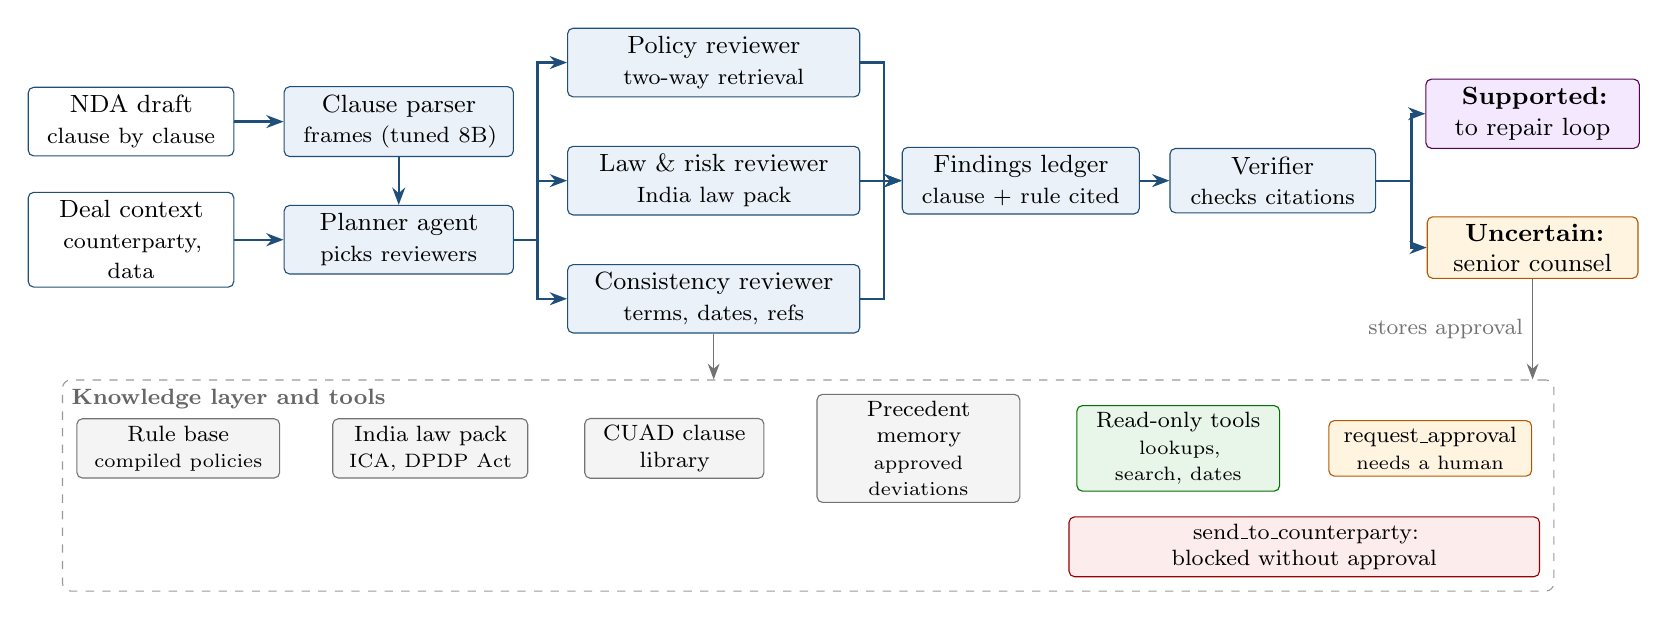
\begin{tikzpicture}
% inputs
\node[box,fill=white,text width=2.4cm] (nda) at (0,0.75) {NDA draft\\\footnotesize clause by clause};
\node[box,fill=white,text width=2.4cm] (ctx) at (0,-0.75) {Deal context\\\footnotesize counterparty, data};
% parser + planner
\node[box,text width=2.7cm] (parse) at (3.4,0.75) {Clause parser\\\footnotesize frames (tuned 8B)};
\node[box,text width=2.7cm] (plan) at (3.4,-0.75) {Planner agent\\\footnotesize picks reviewers};
% reviewers
\node[box,text width=3.5cm] (r1) at (7.4,1.5) {Policy reviewer\\\footnotesize two-way retrieval};
\node[box,text width=3.5cm] (r2) at (7.4,0) {Law \& risk reviewer\\\footnotesize India law pack};
\node[box,text width=3.5cm] (r3) at (7.4,-1.5) {Consistency reviewer\\\footnotesize terms, dates, refs};
% ledger, verifier
\node[box,text width=2.8cm] (led) at (11.3,0) {Findings ledger\\\footnotesize clause + rule cited};
\node[box,text width=2.4cm] (ver) at (14.5,0) {Verifier\\\footnotesize checks citations};
% outputs
\node[spec,text width=2.5cm,font=\small] (rep) at (17.8,0.85) {\textbf{Supported:}\\to repair loop};
\node[tool,text width=2.5cm,font=\small] (hum) at (17.8,-0.85) {\textbf{Uncertain:}\\senior counsel};
% speculation
% arrows main
\draw[arr] (nda) -- (parse);
\draw[arr] (ctx) -- (plan);
\draw[arr] (parse) -- (plan);
\draw[arr] (plan.east) -- ++(0.3,0) |- (r1.west);
\draw[arr] (plan.east) -- ++(0.3,0) |- (r2.west);
\draw[arr] (plan.east) -- ++(0.3,0) |- (r3.west);
\draw[arr] (r1.east) -- ++(0.3,0) |- (led.west);
\draw[arr] (r2.east) -- (led.west);
\draw[arr] (r3.east) -- ++(0.3,0) |- (led.west);
\draw[arr] (led) -- (ver);
\draw[arr] (ver.east) -- ++(0.45,0) |- (rep.west);
\draw[arr] (ver.east) -- ++(0.45,0) |- (hum.west);
% support layer
\node[kb,text width=2.4cm] (kb1) at (0.6,-3.4) {Rule base\\\scriptsize compiled policies};
\node[kb,text width=2.3cm] (kb2) at (3.8,-3.4) {India law pack\\\scriptsize ICA, DPDP Act};
\node[kb,text width=2.1cm] (kb3) at (6.9,-3.4) {CUAD clause\\library};
\node[kb,text width=2.4cm] (kb4) at (10.0,-3.4) {Precedent memory\\\scriptsize approved deviations};
\node[ok,text width=2.4cm] (t1) at (13.3,-3.4) {Read-only tools\\\scriptsize lookups, search, dates};
\node[tool,text width=2.4cm] (t2) at (16.5,-3.4) {request\_approval\\\scriptsize needs a human};
\node[bad,text width=5.8cm] (t3) at (14.9,-4.65) {send\_to\_counterparty: blocked without approval};
\begin{scope}[on background layer]
\node[draw=black!40,dashed,rounded corners=3pt,fit=(kb1)(kb4)(t1)(t2)(t3),inner sep=5pt] (sup) {};
\end{scope}
\node[font=\footnotesize\bfseries,black!60,anchor=north west] at (sup.north west) {Knowledge layer and tools};
\draw[garr] (r3.south) -- (r3.south |- sup.north);
\draw[garr] (hum.south) -- (hum.south |- sup.north) node[pos=0.5,left,font=\footnotesize]{stores approval};
\end{tikzpicture}}
\caption{Detection pipeline (RQ1). Blue boxes are LLM agents (same backbone in every system we compare). Green tools are read-only, orange needs human approval, and red is never allowed without approval. Supported findings go on to the red-team and repair loop in Figure~3.}
\end{figure}

\textbf{How it works.} The \emph{clause parser} turns each clause into an \emph{obligation frame} \{party, action, object, condition, duration, exception\}, so numbers and conditions can be compared exactly rather than by text similarity. Offline, a \emph{policy compiler} turns each company's prose policies into a rule base, where every rule has an ID, an applicability condition (e.g.\ \texttt{vendor AND personal\_data}), a requirement and its source text. The \emph{planner} picks reviewers based on the deal and the clause types present. Three reviewers call tools and write findings to a shared ledger. The \emph{verifier} keeps a finding only if both citations (NDA clause and rule or statute) support it, and sends uncertain or approval-gated cases to a senior lawyer. Approved deviations go into \emph{precedent memory}, so the same question is not escalated twice.

\begin{figure}[tb]
\centering
\resizebox{0.66\textwidth}{!}{%
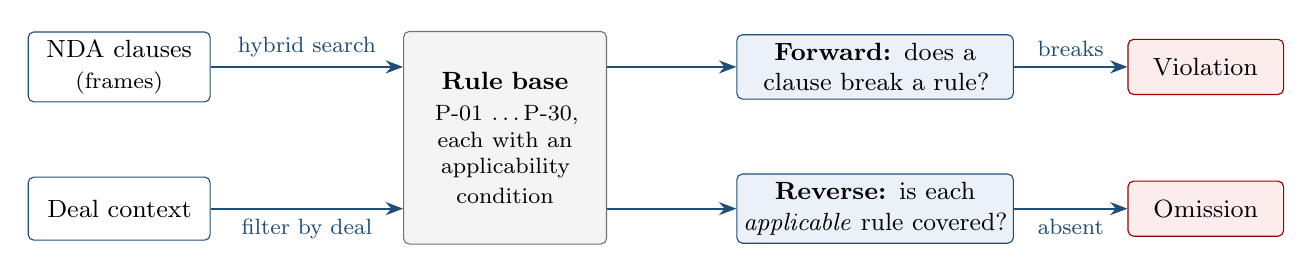
\begin{tikzpicture}
\node[box,fill=white,text width=2.1cm] (cl) at (0,0.9) {NDA clauses\\\footnotesize (frames)};
\node[box,fill=white,text width=2.1cm] (dc) at (0,-0.9) {Deal context};
\node[kb,text width=2.4cm,minimum height=2.7cm,font=\small] (rb) at (4.9,0) {\textbf{Rule base}\\[2pt]\footnotesize P-01 \ldots P-30,\\each with an\\applicability\\condition};
\node[box,text width=3.3cm] (fw) at (9.6,0.9) {\textbf{Forward:} does a clause break a rule?};
\node[box,text width=3.3cm] (rv) at (9.6,-0.9) {\textbf{Reverse:} is each \emph{applicable} rule covered?};
\node[bad,text width=1.8cm,font=\small] (vi) at (13.8,0.9) {Violation};
\node[bad,text width=1.8cm,font=\small] (om) at (13.8,-0.9) {Omission};
\draw[arr] (cl) -- node[above,font=\footnotesize]{hybrid search} (rb.west |- cl);
\draw[arr] (dc) -- node[below,font=\footnotesize]{filter by deal} (rb.west |- dc);
\draw[arr] (rb.east |- fw) -- (fw);
\draw[arr] (rb.east |- rv) -- (rv);
\draw[arr] (fw) -- node[above,font=\footnotesize]{breaks} (vi);
\draw[arr] (rv) -- node[below,font=\footnotesize]{absent} (om);
\end{tikzpicture}}
\caption{Two-way retrieval. The reverse path is the only way to find a \emph{missing} clause, and the deal filter stops rules that don't apply to this deal from firing.}
\end{figure}

\begin{figure}[tb]
\centering
\resizebox{\textwidth}{!}{%
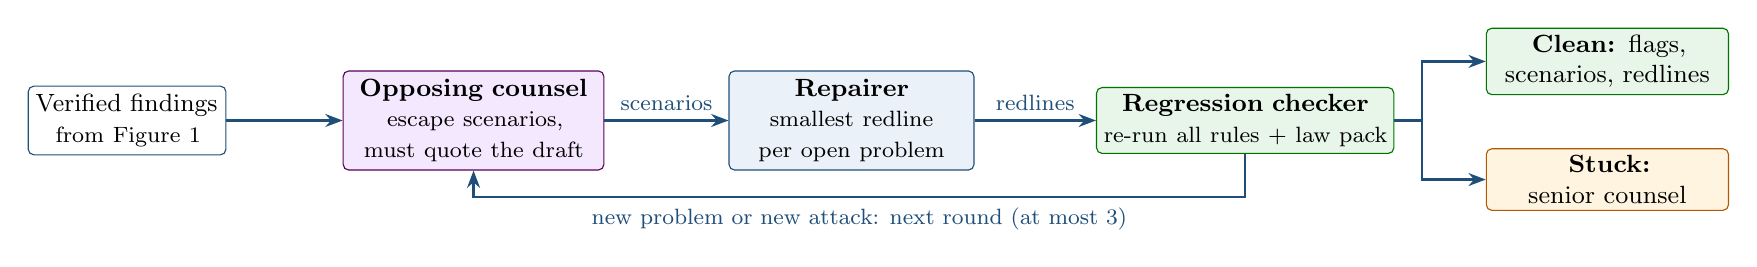
\begin{tikzpicture}[x=1cm,y=1cm]
\node[box,fill=white,text width=2.3cm] (in) at (0,0) {Verified findings\\\footnotesize from Figure~1};
\node[spec,text width=3.1cm] (att) at (4.4,0) {\textbf{Opposing counsel}\\\footnotesize escape scenarios, must quote the draft};
\node[box,text width=2.9cm] (rep) at (9.2,0) {\textbf{Repairer}\\\footnotesize smallest redline per open problem};
\node[ok,text width=3.6cm,font=\small] (reg) at (14.2,0) {\textbf{Regression checker}\\\footnotesize re-run all rules + law pack};
\node[ok,text width=2.9cm,font=\small] (out) at (18.8,0.75) {\textbf{Clean:} flags, scenarios, redlines};
\node[tool,text width=2.9cm,font=\small] (hum) at (18.8,-0.75) {\textbf{Stuck:}\\senior counsel};
\draw[arr] (in) -- (att);
\draw[arr] (att) -- node[above,font=\footnotesize]{scenarios} (rep);
\draw[arr] (rep) -- node[above,font=\footnotesize]{redlines} (reg);
\draw[arr] (reg.east) -- ++(0.35,0) |- (out.west);
\draw[arr] (reg.east) -- ++(0.35,0) |- (hum.west);
\draw[arr] (reg.south) -- ++(0,-0.55) -| node[pos=0.25,below,font=\footnotesize]{new problem or new attack: next round (at most 3)} (att.south);
\end{tikzpicture}}
\caption{Red-team and repair loop (RQ2), borrowed from counterexample-guided refinement (formal verification) and regression testing (program repair). At most 3 rounds. Final scores use gold original clauses, held-out checks and a validated judge, never this loop's own checker.}
\end{figure}

\textbf{RAG design.} Retrieval combines BM25 and dense search with a cross-encoder reranker, so legal terms like ``indemnify'' match exactly. Policies are chunked by rule rather than by fixed size, so an exception stays with its rule. A one-hop cross-reference graph pulls in linked approval rules and statutory exceptions. Because Gemini can read a whole 40k-token pack, we do not assume RAG is needed. We \emph{measure} it with a policy-size sweep at 40k and 150k tokens (400k if time allows).

\textbf{Red-team and repair loop.} Fixes interact: lengthening a term to satisfy one rule can break another rule's maximum, and a non-solicit added to protect staff can create a restraint-of-trade risk. Checklists also miss what the other side could \emph{exploit}, such as a residuals clause or a definition that leaves out oral disclosures. So after detection, an \emph{opposing-counsel agent} writes escape scenarios that must quote the draft and pass the verifier. A \emph{repairer} writes the smallest clause-level redline for each open problem, and a \emph{regression checker} re-runs the whole rule base and law pack on the edited draft. The loop stops when nothing new is found, or escalates when the budget runs out or two rules can't both be met. Ground truth is exact: every planted defect was made by editing an original clause, so \emph{the original is the gold repair}, and ContractNLI's expert labels mark classic loopholes (e.g.\ \emph{permissible development of similar information}).

%================ 5 =================
\section{The five capabilities: why each is needed and how we measure it}
\begin{table}[H]\small
\begin{tabularx}{\textwidth}{@{}p{2.1cm}LL@{}}
\toprule
\textbf{Capability} & \textbf{Why this problem needs it} & \textbf{How we measure it} \\
\midrule
Fine-tuning & One QLoRA Llama-3.1-8B for clause tags (CUAD), ContractNLI checks and obligation frames. The regression checker re-runs every rule after every repair round, so checks must be cheap, local and consistent. & CUAD tag F1; ContractNLI acc./macro-F1 (12 trained, 5 held-out checks); frame field accuracy on 300 gold frames; tuned vs untuned vs prompted Gemini \\
RAG & An omission check must find \emph{every} applicable rule, cite it exactly and stay cheap as the policy corpus grows. & Applicable-rule recall@k, omission recall, nDCG@10, policy-size sweep vs long context \\
Reasoning & Deciding whether a rule applies to this deal; reasoning about how a clause can be exploited; planning repairs under interacting rules; verification. & Accuracy of every intermediate applicability decision vs gold; loophole recall; regression rate; verifier precision; cause of each miss \\
Agentic & Planner and reviewers; an \textbf{attacker vs repairer loop} with a stopping rule; shared ledger, precedent memory, hand-off to a senior lawyer. & Loop vs one-shot repair vs self-refine; rounds to convergence; planner vs fixed pipeline; hand-off precision/recall \\
Tool calling & Exact bookkeeping (terms, dates, cross-references), rule/statute/approval lookups, applying redlines, full re-checks, gated actions. & Tool precision/recall vs gold tool sets per defect type, argument validity, recovery from 10\% injected errors, \textbf{unsafe action rate (target 0)} \\
\bottomrule
\end{tabularx}
\end{table}

%================ 6 =================
\section{Dataset and evaluation environment: PolicyNDA}
\begin{itemize}
\item \textbf{NDAs:} ContractNLI (607 real NDAs, split 423/61/123, CC BY 4.0). \textbf{Clause library:} CUAD (510 contracts, 41 clause types).
\item \textbf{Company policy packs (we write):} 3 fictional Indian companies, each with $\sim$30 NDA rules buried in $\sim$40k tokens of realistic prose. They are written by teammates who do not build the system, and the gold rule lists are kept separate.
\item \textbf{India law pack:} $\sim$15 clear-cut provisions (ICA s.23/27/28, DPDP Act 2023, Arbitration Act seat rules, Specific Relief Act), each checked by two teammates.
\item \textbf{Ground truth without circularity:} about 60\% of the rules are anchored to ContractNLI's 17 expert-labelled checks (e.g.\ ``vendor NDAs must require return of information'' $\leftrightarrow$ \emph{return of confidential information}). So each real NDA's \emph{natural} omissions and violations are already labelled by legal experts. The remaining field rules (governing law, term length) are hand-labelled by two annotators, with Cohen's $\kappa$ reported.
\item \textbf{Planted defects on top:} violations, omissions, approval-gated deviations, statutory risks, internal inconsistencies, prompt-injection text, and \emph{distractors} (rules that look relevant but don't apply), giving 2--4 per NDA. About 25\% of NDAs get only distractors, so we can measure false alarms.
\item \textbf{Loopholes and gold repairs (RQ2):} natural loopholes come from ContractNLI's loophole checks, and 1--2 more are planted in half of the test NDAs (residuals clauses, carve-outs with no time limit). Gold repairs are the original clauses behind planted defects, plus gold frames for natural defects on 40 NDAs.
\end{itemize}

%================ 7 =================
\section{Evaluation plan}
\textbf{Two-stage backbone.} Stage 1 runs everything on \textbf{Llama-3.1-8B} served free on Kaggle GPUs. Stage 2 confirms the main systems on \textbf{Gemini 3.8 Flash}. All systems in a comparison use the same backbone. Long-context runs and the policy-size sweep need Gemini, because a T4 GPU cannot hold a 40k-token prompt.

\begin{table}[H]\small
\begin{tabularx}{\textwidth}{@{}>{\raggedright\arraybackslash}p{2.3cm}L@{}}
\toprule
\textbf{RQ1 baselines} & B1 long context (whole pack in one prompt) $\cdot$ B2 naive RAG (fixed chunks, forward only) $\cdot$ B3 single agent with tools $\cdot$ B4 exhaustive per-rule checking (PolicyGuard-style) \\
\textbf{RQ2 baselines} & R1 one-shot ``fix all issues'' repair $\cdot$ R2 Self-Refine (no attacker, no full re-check). Both start from the same findings with the same token budget. \\
\textbf{Ablations} (one change each) & no reverse retrieval (clean RQ1 test) $\cdot$ no deal filter $\cdot$ no frames $\cdot$ no verifier $\cdot$ planner $\rightarrow$ fixed pipeline $\cdot$ untuned model $\cdot$ no cross-reference graph $\cdot$ no memory $\cdot$ loop: no attacker / no regression check / 1 vs 3 rounds / attacker on a different model $\cdot$ \textbf{local-first cascade} (Gemini only for unsure or high-severity checks) vs all-Gemini \\
\textbf{Detection} & Recall, precision and F1 per defect type; \textbf{omission recall}; false alarms per NDA. A finding counts only if both citations are correct. Natural and planted defects are reported separately. \\
\textbf{Repair loop} & Remaining defects and loopholes per NDA; \textbf{regression rate} (new violations per redline); repair success vs gold; attacker loophole recall and precision; edit size; rounds; blind acceptance (two raters, $\kappa$) \\
\textbf{Cost} & \$ per NDA; share of checks escalated; misses by severity vs escalation rate \\
\textbf{Safety} & Unsafe/unapproved action rate (target 0), including prompt-injection text inside NDAs; hand-off precision and recall \\
\textbf{Rigour} & Bootstrap 95\% CIs and McNemar's test. An LLM judge is used only for explanation quality, validated against 100 human labels (Cohen's $\kappa$). Five worked qualitative cases and a table of misses by cause. \\
\bottomrule
\end{tabularx}
\end{table}

%================ 8 =================
\section{Expected novelty}
\begin{enumerate}
\item \textbf{PolicyNDA}, the first \emph{open} benchmark for checking NDAs against company policy. It covers omissions and deal-specific applicability, with ground truth anchored to expert labels.
\item \textbf{Applicability-aware two-way retrieval}, compared honestly against exhaustive per-rule checking and against long context as the policy corpus grows.
\item \textbf{A counterexample-guided red-team and repair loop} for contract drafting. An opposing-counsel agent attacks, a repairer fixes and a regression checker guards every edit. This adds the repair, adversary and cross-rule checking that PolicyGuard lacks, measured against exact gold repairs.
\end{enumerate}

%================ 9 =================
\section{Safety plan}
\begin{itemize}
\item Only public NDAs and synthetic policies, so no client or personal data. Llama runs locally; only public or synthetic text goes to the Gemini API, on the paid tier.
\item Gated actions: \texttt{request\_approval} needs human confirmation, and \texttt{send\_to\_counterparty} is a mock that is blocked without approval. Misuse is measured, including under prompt injection.
\item Redlines are suggestions the consultant accepts or rejects; nothing is sent or signed. Escape scenarios are internal analysis for the company's own lawyer.
\item The output is decision support with citations, not legal advice. No team member is a lawyer, so statutory flags are worded as ``risk under s.27'' and the law pack is small, cited and dated.
\end{itemize}

%================ 10 =================
\section{Compute plan}
\begin{table}[H]\small
\begin{tabularx}{\textwidth}{@{}LXr@{}}
\toprule
\textbf{Item} & \textbf{Resource} & \textbf{Estimate} \\
\midrule
QLoRA Llama-3.1-8B, multi-task, $\sim$18k examples, 2 runs & Kaggle T4 (free) & $\approx$16 GPU-h \\
Tuned-model inference (ContractNLI test, regression checks in the loop) & Kaggle T4, vLLM & $\approx$8 GPU-h \\
Stage 1: all systems, the loop and ablations on Llama-8B, 123 NDAs, 2 seeds & Kaggle 2$\times$T4, vLLM & $\approx$35 GPU-h, \$0 \\
Stage 2: Full, B1, B2, B4 and 2 RQ1 ablations, 123 NDAs ($\approx$18M in / 4M out, context-cached) & Gemini 3.8 Flash, Batch API & $\approx$\$15 \\
RQ2 loop, R1, R2; policy-size sweep; local-first loop and ablation checks on 40 NDAs & Gemini 3.8 Flash, Batch API & $\approx$\$22 \\
Silver frames, policy prose (Flash); policy compilation (Pro, once) & Gemini, Batch API & $\approx$\$10 \\
\midrule
\textbf{Total} & & \textbf{$\approx$60 GPU-h, $\approx$\$45} \\
\bottomrule
\end{tabularx}
\end{table}
\vspace{-4pt}
{\small Prices from the official Gemini pricing page (2 Oct 2026): 3.8 Flash costs \$0.75 in / \$3.75 out per million tokens until 31 Dec 2026, then double, so the API total is $\approx$\$85 if stage 2 runs after that date. 60 GPU-hours is about two weeks of Kaggle's free quota.}

%================ 11 =================
\section{Risks and fallback plan}
\begin{table}[H]\footnotesize
\begin{tabularx}{\textwidth}{@{}LL@{}}
\toprule
\textbf{Risk} & \textbf{Fallback} \\
\midrule
Scope too large for the time & RQ1 and the loop with its regression checker are the core. Drop the different-model attacker first, then cap the loop at 2 rounds. \\
Loop games its own checker or invents loopholes & Scores use only gold originals, held-out checks and a validated judge; scenarios must quote the draft and pass the verifier. \\
Long context or exhaustive checking matches our retrieval & Report it; the benchmark, omission results and cost gap remain contributions. \\
Llama-8B too weak for tool use & Constrained JSON decoding; hosted Llama-70B for stage 1. \\
Gains come from memorised ContractNLI labels & 5 checks are held out of fine-tuning and reported separately. \\
Loop doesn't beat self-refine & Report it: the adversary isn't needed; the regression checker is still measured. \\
Unrealistic policies or law errors & Model policies on public corporate policies; realism check by a teammate; two-person law check. \\
\bottomrule
\end{tabularx}
\end{table}

\vspace{-8pt}
{\scriptsize\textbf{Key references.} Koreeda \& Manning, ContractNLI (2021) $\cdot$ Hendrycks et al., CUAD (2021) $\cdot$ CLAUSE (arXiv:2511.00340) $\cdot$ ContractScrub (arXiv:2608.20204) $\cdot$ ContractEval (arXiv:2508.03080) $\cdot$ PolicyGuard (arXiv:2606.32004) $\cdot$ CEGAR (Clarke et al. 2000) $\cdot$ Madaan et al., Self-Refine (2023) $\cdot$ LegalSim (arXiv:2510.03405) $\cdot$ AgentCourt (arXiv:2408.08089) $\cdot$ QLoRA (2023).}

\end{document}
